% \tikzset{every picture/.style={line width=0.75pt}} %set default line width to 0.75pt        

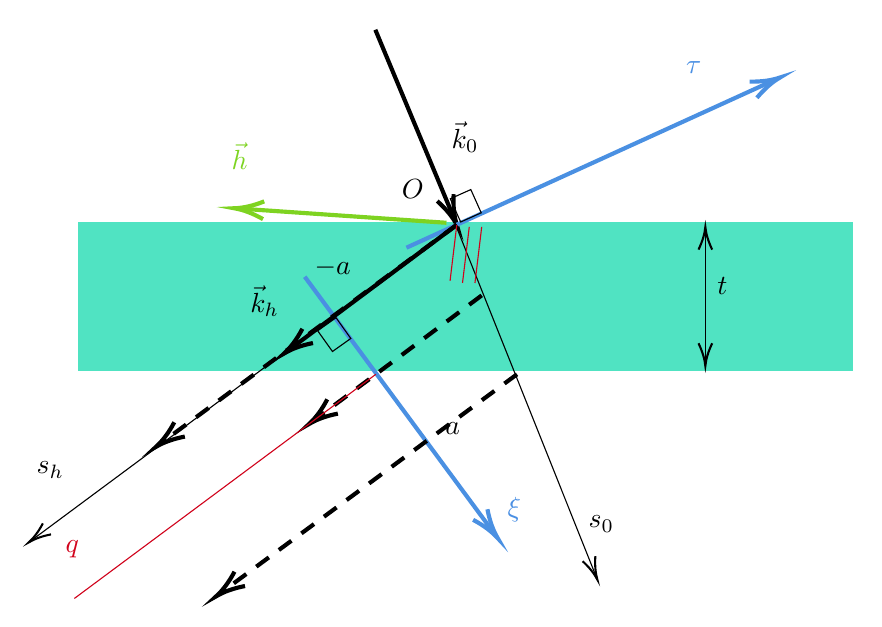
\begin{tikzpicture}[x=0.75pt,y=0.75pt,yscale=-1,xscale=1]
%uncomment if require: \path (0,300); %set diagram left start at 0, and has height of 300

%Shape: Rectangle [id:dp4659059300300452] 
\draw  [draw opacity=0][fill={rgb, 255:red, 80; green, 227; blue, 194 }  ,fill opacity=1 ][line width=0.75]  (136.25,107.5) -- (509.75,107.5) -- (509.75,179.5) -- (136.25,179.5) -- cycle ;
%Straight Lines [id:da16285737660398936] 
\draw [line width=1.5]    (279.5,15) -- (317.59,106.23) ;
\draw [shift={(318.75,109)}, rotate = 247.34] [color={rgb, 255:red, 0; green, 0; blue, 0 }  ][line width=1.5]    (14.21,-4.28) .. controls (9.04,-1.82) and (4.3,-0.39) .. (0,0) .. controls (4.3,0.39) and (9.04,1.82) .. (14.21,4.28)   ;
%Straight Lines [id:da0633156187913293] 
\draw [color={rgb, 255:red, 74; green, 144; blue, 226 }  ,draw opacity=1 ][line width=1.5]    (294.5,120) -- (471.77,39.24) ;
\draw [shift={(474.5,38)}, rotate = 515.51] [color={rgb, 255:red, 74; green, 144; blue, 226 }  ,draw opacity=1 ][line width=1.5]    (14.21,-4.28) .. controls (9.04,-1.82) and (4.3,-0.39) .. (0,0) .. controls (4.3,0.39) and (9.04,1.82) .. (14.21,4.28)   ;
%Straight Lines [id:da5835744267291234] 
\draw [color={rgb, 255:red, 74; green, 144; blue, 226 }  ,draw opacity=1 ][line width=1.5]    (245.5,134) -- (336.72,257.59) ;
\draw [shift={(338.5,260)}, rotate = 233.57] [color={rgb, 255:red, 74; green, 144; blue, 226 }  ,draw opacity=1 ][line width=1.5]    (14.21,-4.28) .. controls (9.04,-1.82) and (4.3,-0.39) .. (0,0) .. controls (4.3,0.39) and (9.04,1.82) .. (14.21,4.28)   ;
%Straight Lines [id:da5813004556859225] 
\draw [line width=1.5]  [dash pattern={on 5.63pt off 4.5pt}]  (330.75,143) -- (249.91,203.21) ;
\draw [shift={(247.5,205)}, rotate = 323.32] [color={rgb, 255:red, 0; green, 0; blue, 0 }  ][line width=1.5]    (14.21,-4.28) .. controls (9.04,-1.82) and (4.3,-0.39) .. (0,0) .. controls (4.3,0.39) and (9.04,1.82) .. (14.21,4.28)   ;
%Straight Lines [id:da9494728644400778] 
\draw [color={rgb, 255:red, 126; green, 211; blue, 33 }  ,draw opacity=1 ][line width=1.5]    (313.75,108) -- (214.49,101.2) ;
\draw [shift={(211.5,101)}, rotate = 363.91999999999996] [color={rgb, 255:red, 126; green, 211; blue, 33 }  ,draw opacity=1 ][line width=1.5]    (14.21,-4.28) .. controls (9.04,-1.82) and (4.3,-0.39) .. (0,0) .. controls (4.3,0.39) and (9.04,1.82) .. (14.21,4.28)   ;
%Straight Lines [id:da8605907310239256] 
\draw [line width=1.5]  [dash pattern={on 5.63pt off 4.5pt}]  (318.75,109) -- (176.16,214.22) ;
\draw [shift={(173.75,216)}, rotate = 323.58000000000004] [color={rgb, 255:red, 0; green, 0; blue, 0 }  ][line width=1.5]    (14.21,-4.28) .. controls (9.04,-1.82) and (4.3,-0.39) .. (0,0) .. controls (4.3,0.39) and (9.04,1.82) .. (14.21,4.28)   ;
%Straight Lines [id:da5375852608603029] 
\draw [line width=1.5]  [dash pattern={on 5.63pt off 4.5pt}]  (347.75,181) -- (205.16,286.22) ;
\draw [shift={(202.75,288)}, rotate = 323.58000000000004] [color={rgb, 255:red, 0; green, 0; blue, 0 }  ][line width=1.5]    (14.21,-4.28) .. controls (9.04,-1.82) and (4.3,-0.39) .. (0,0) .. controls (4.3,0.39) and (9.04,1.82) .. (14.21,4.28)   ;
%Straight Lines [id:da19735589184858027] 
\draw    (293,46) -- (385.76,278.14) ;
\draw [shift={(386.5,280)}, rotate = 248.22] [color={rgb, 255:red, 0; green, 0; blue, 0 }  ][line width=0.75]    (10.93,-3.29) .. controls (6.95,-1.4) and (3.31,-0.3) .. (0,0) .. controls (3.31,0.3) and (6.95,1.4) .. (10.93,3.29)   ;
%Straight Lines [id:da9826081768178245] 
\draw    (318.75,109) -- (114.11,260.81) ;
\draw [shift={(112.5,262)}, rotate = 323.43] [color={rgb, 255:red, 0; green, 0; blue, 0 }  ][line width=0.75]    (10.93,-3.29) .. controls (6.95,-1.4) and (3.31,-0.3) .. (0,0) .. controls (3.31,0.3) and (6.95,1.4) .. (10.93,3.29)   ;
%Straight Lines [id:da6014347424725826] 
\draw [color={rgb, 255:red, 208; green, 2; blue, 27 }  ,draw opacity=1 ]   (279.75,181) -- (134.5,289) ;
%Straight Lines [id:da41688299688679864] 
\draw [line width=1.5]    (318.75,109) -- (237.91,169.21) ;
\draw [shift={(235.5,171)}, rotate = 323.32] [color={rgb, 255:red, 0; green, 0; blue, 0 }  ][line width=1.5]    (14.21,-4.28) .. controls (9.04,-1.82) and (4.3,-0.39) .. (0,0) .. controls (4.3,0.39) and (9.04,1.82) .. (14.21,4.28)   ;
%Straight Lines [id:da2945221843089698] 
\draw [color={rgb, 255:red, 208; green, 2; blue, 27 }  ,draw opacity=1 ]   (318.75,109) -- (315.5,136) ;
%Straight Lines [id:da2409863293898824] 
\draw [color={rgb, 255:red, 208; green, 2; blue, 27 }  ,draw opacity=1 ]   (330.75,110) -- (327.5,137) ;
%Straight Lines [id:da6213466215159829] 
\draw [color={rgb, 255:red, 208; green, 2; blue, 27 }  ,draw opacity=1 ]   (324.75,110) -- (321.5,137) ;
%Shape: Rectangle [id:dp6858543372227281] 
\draw   (315.61,96.43) -- (325.5,92) -- (330.52,103.19) -- (320.62,107.63) -- cycle ;
%Shape: Rectangle [id:dp16408028713981904] 
\draw   (251.73,160.03) -- (260.56,153.74) -- (267.68,163.73) -- (258.85,170.02) -- cycle ;
%Straight Lines [id:da6941190929293435] 
\draw    (438.5,112) -- (438.5,175) ;
\draw [shift={(438.5,177)}, rotate = 270] [color={rgb, 255:red, 0; green, 0; blue, 0 }  ][line width=0.75]    (10.93,-3.29) .. controls (6.95,-1.4) and (3.31,-0.3) .. (0,0) .. controls (3.31,0.3) and (6.95,1.4) .. (10.93,3.29)   ;
\draw [shift={(438.5,110)}, rotate = 90] [color={rgb, 255:red, 0; green, 0; blue, 0 }  ][line width=0.75]    (10.93,-3.29) .. controls (6.95,-1.4) and (3.31,-0.3) .. (0,0) .. controls (3.31,0.3) and (6.95,1.4) .. (10.93,3.29)   ;

% Text Node
\draw (291,86) node [anchor=north west][inner sep=0.75pt]   [align=left] {$\displaystyle O$};
% Text Node
\draw (428,29) node [anchor=north west][inner sep=0.75pt]   [align=left] {$\displaystyle \textcolor[rgb]{0.29,0.56,0.89}{\tau }$};
% Text Node
\draw (342,239) node [anchor=north west][inner sep=0.75pt]   [align=left] {$\displaystyle \textcolor[rgb]{0.29,0.56,0.89}{\xi }$};
% Text Node
\draw (249,124) node [anchor=north west][inner sep=0.75pt]   [align=left] {$\displaystyle -a$};
% Text Node
\draw (312,203) node [anchor=north west][inner sep=0.75pt]   [align=left] {$\displaystyle a$};
% Text Node
\draw (315,58) node [anchor=north west][inner sep=0.75pt]   [align=left] {$\displaystyle \vec{k}_{0}$};
% Text Node
\draw (381,248) node [anchor=north west][inner sep=0.75pt]   [align=left] {$\displaystyle s_{0}$};
% Text Node
\draw (115,222) node [anchor=north west][inner sep=0.75pt]   [align=left] {$\displaystyle s_{h}$};
% Text Node
\draw (129,260) node [anchor=north west][inner sep=0.75pt]   [align=left] {$\displaystyle \textcolor[rgb]{0.82,0.01,0.11}{q}$};
% Text Node
\draw (218,137) node [anchor=north west][inner sep=0.75pt]   [align=left] {$\displaystyle \vec{k}_{h}$};
% Text Node
\draw (209,68) node [anchor=north west][inner sep=0.75pt]  [color={rgb, 255:red, 126; green, 211; blue, 33 }  ,opacity=1 ] [align=left] {$\displaystyle \vec{\textcolor[rgb]{0.49,0.83,0.13}{h}}$};
% Text Node
\draw (443,133) node [anchor=north west][inner sep=0.75pt]   [align=left] {$\displaystyle t$};


\end{tikzpicture}
